\documentclass[10pt,letterpaper]{article}
%\usepackage{tools}
\usepackage{geometry}
\usepackage{amsmath}
\usepackage{xepersian}
\usepackage{enumitem}
%\settextfont{B Nazanin}
\usepackage{lipsum}
\setlength{\parskip}{3mm}
\setlength{\parindent}{0mm}
\begin{document}
\Large
\begin{center}
به نام او

امتحان میانترم درس شبکه های مخابراتی

مدت زمان: 90 دقیقه

\hrulefill
\end{center}
سوال 1) درستی یا نادرستی هر یک از گزاره های زیر را با بیان دلایل کافی تعیین کنید.

الف) الگوریتم های iBGP و eBGP برای انتقال دادن اطلاعات از \lr{Gateway Router} های هر AS به نودهای داخلی آن مورد استفاده قرار می‌گیرند.

ب) در مکانیزم \lr{Congestion Control} با رویکرد Tahoe و شروع از حالت \lr{Slow Start}، هنگامی که فرستنده برای یک بسته‌ی ارسالی خود 3 پیام ACK تکراری دریافت می کند، مقدار cwnd خود را برابر 1 کرده و به حالت \lr{Fast Recovery} می رود.

پ) \lr{Packet Switching} بدلیل تقسیم بندی زمانی یا فرکانسی طیف و اختصاص دادن همزمان پهنای باند به چند کاربر، نسبت به \lr{Circuit Switching} از دیدگاه کاربری بهینه طیف، بهتر است.

ت) در روش \lr{Virtual Circuit} در لایه‌ی شبکه مانند TCP در لایه‌ی \lr{Transport}، \lr{Connection Setup} به صورت \lr{end-to-end} صورت می‌پذیرد.

ث) در مکانیزم \lr{TCP Flow Control}، هنگامی که گیرنده مقدار rwnd را برابر صفر اعلام می کند، فرستنده در ارسال بعدی 1byte می فرستد.
\newpage
سوال 2) یک کاربر برای مشاهده‌ی صفحه‌ی وب خاصی که شامل 10 تصویر هر یک با حجم 
$
12.5Kbytes
$
است، درخواست می دهد. مطابق شکل زیر بین کاربر و سرور، دو لینک و یک روتر وجود دارد. اگر طول هر لینک 50 کیلومتر، نرخ ارسال روی لینک های 1 و 2 به ترتیب 
$
2000 Kbps
$
 و
$
1000 Kbps
$
و درخواست از نوع 
persistent
باشد، چقدر طول می کشد که کاربر بتواند صفحه‌ی وب را با تمام تصاویر داخل آن دانلود کند؟

(حجم درخواست ها و صفحه‌ی HTTP را ناچیز در نظر بگیرید. همچنین تاخیر صف و پردازش روتر برابر صفر و سرعت نور 
$
2\times 10^8 \text{m/s}
$
است.)
\begin{figure}[htb]
\centering
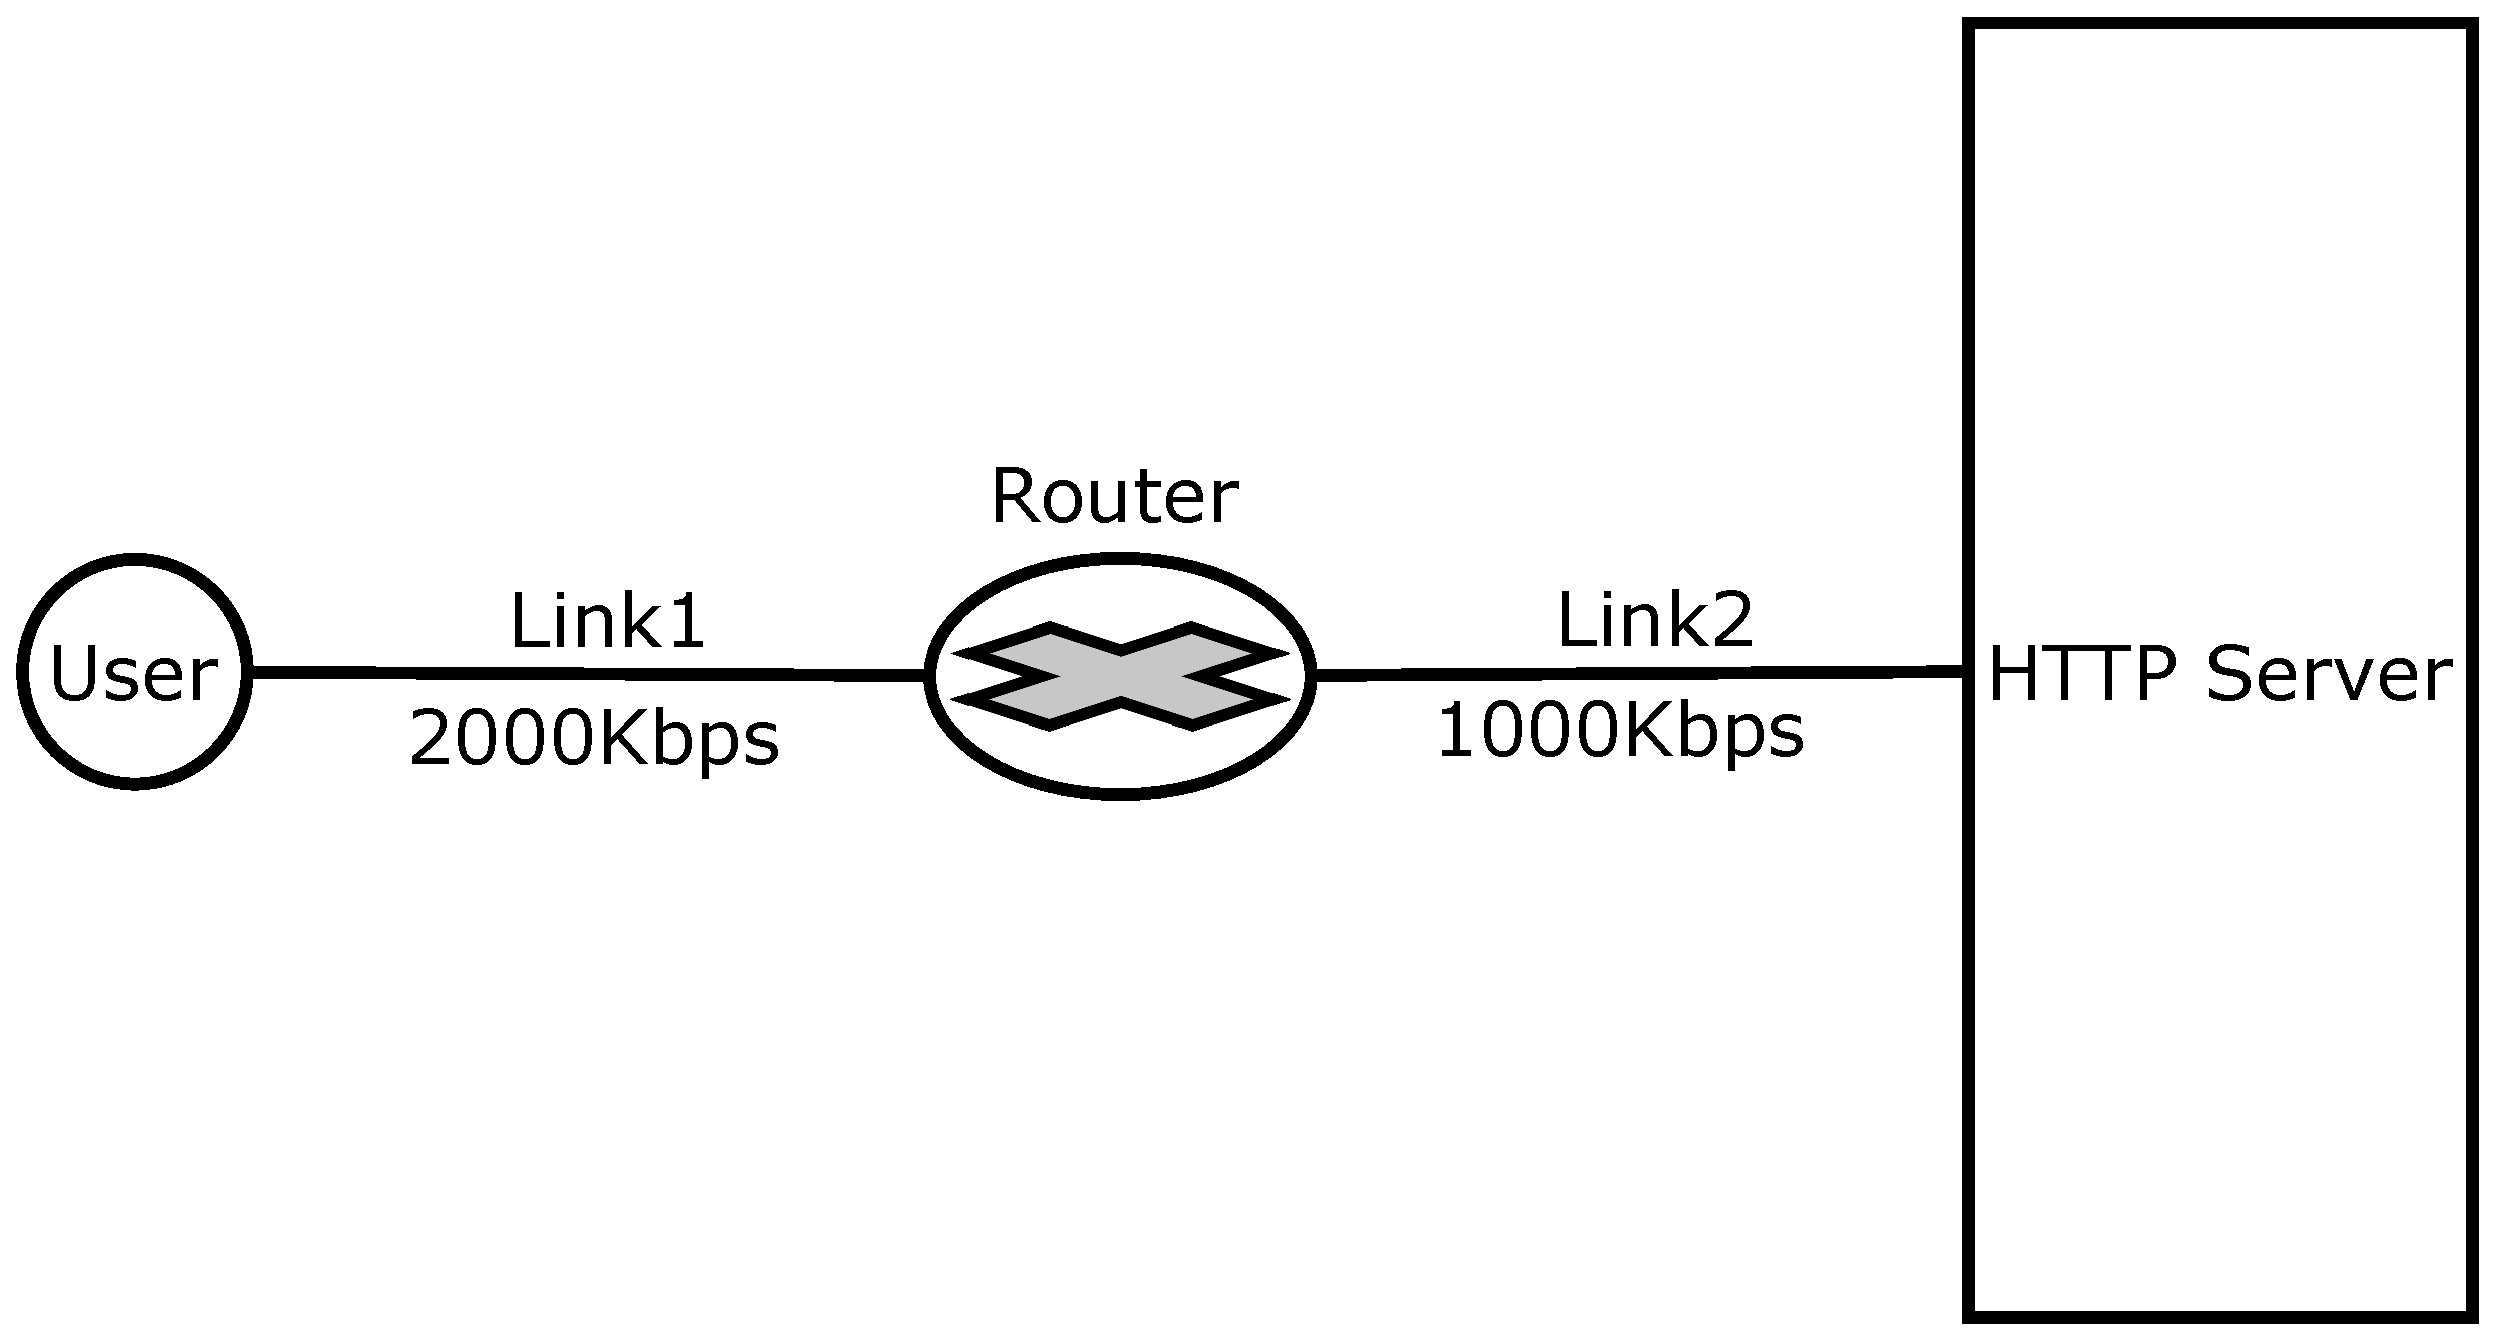
\includegraphics[width=100mm]{Q2.eps}
\end{figure}
\newpage
سوال 3) فرض کنید فرستنده ای، 4 بسته با شماره‌های 0، 1، 2 و 3 را به ترتیب و پشت سر هم ارسال می کند. بسته‌ی شماره‌ی 2 به گیرنده نمیرسد و بسته‌ی شماره‌ی 1 (شماره 3) نیز به مقصد رسیده، ولی ACK آن در کانال از بین می‌رود. توضیح دهید هر یک از الگوریتم های 
GBN
و
SR
چه عملکردی را از خود نشان می دهند.
\begin{figure}[htb]
\centering
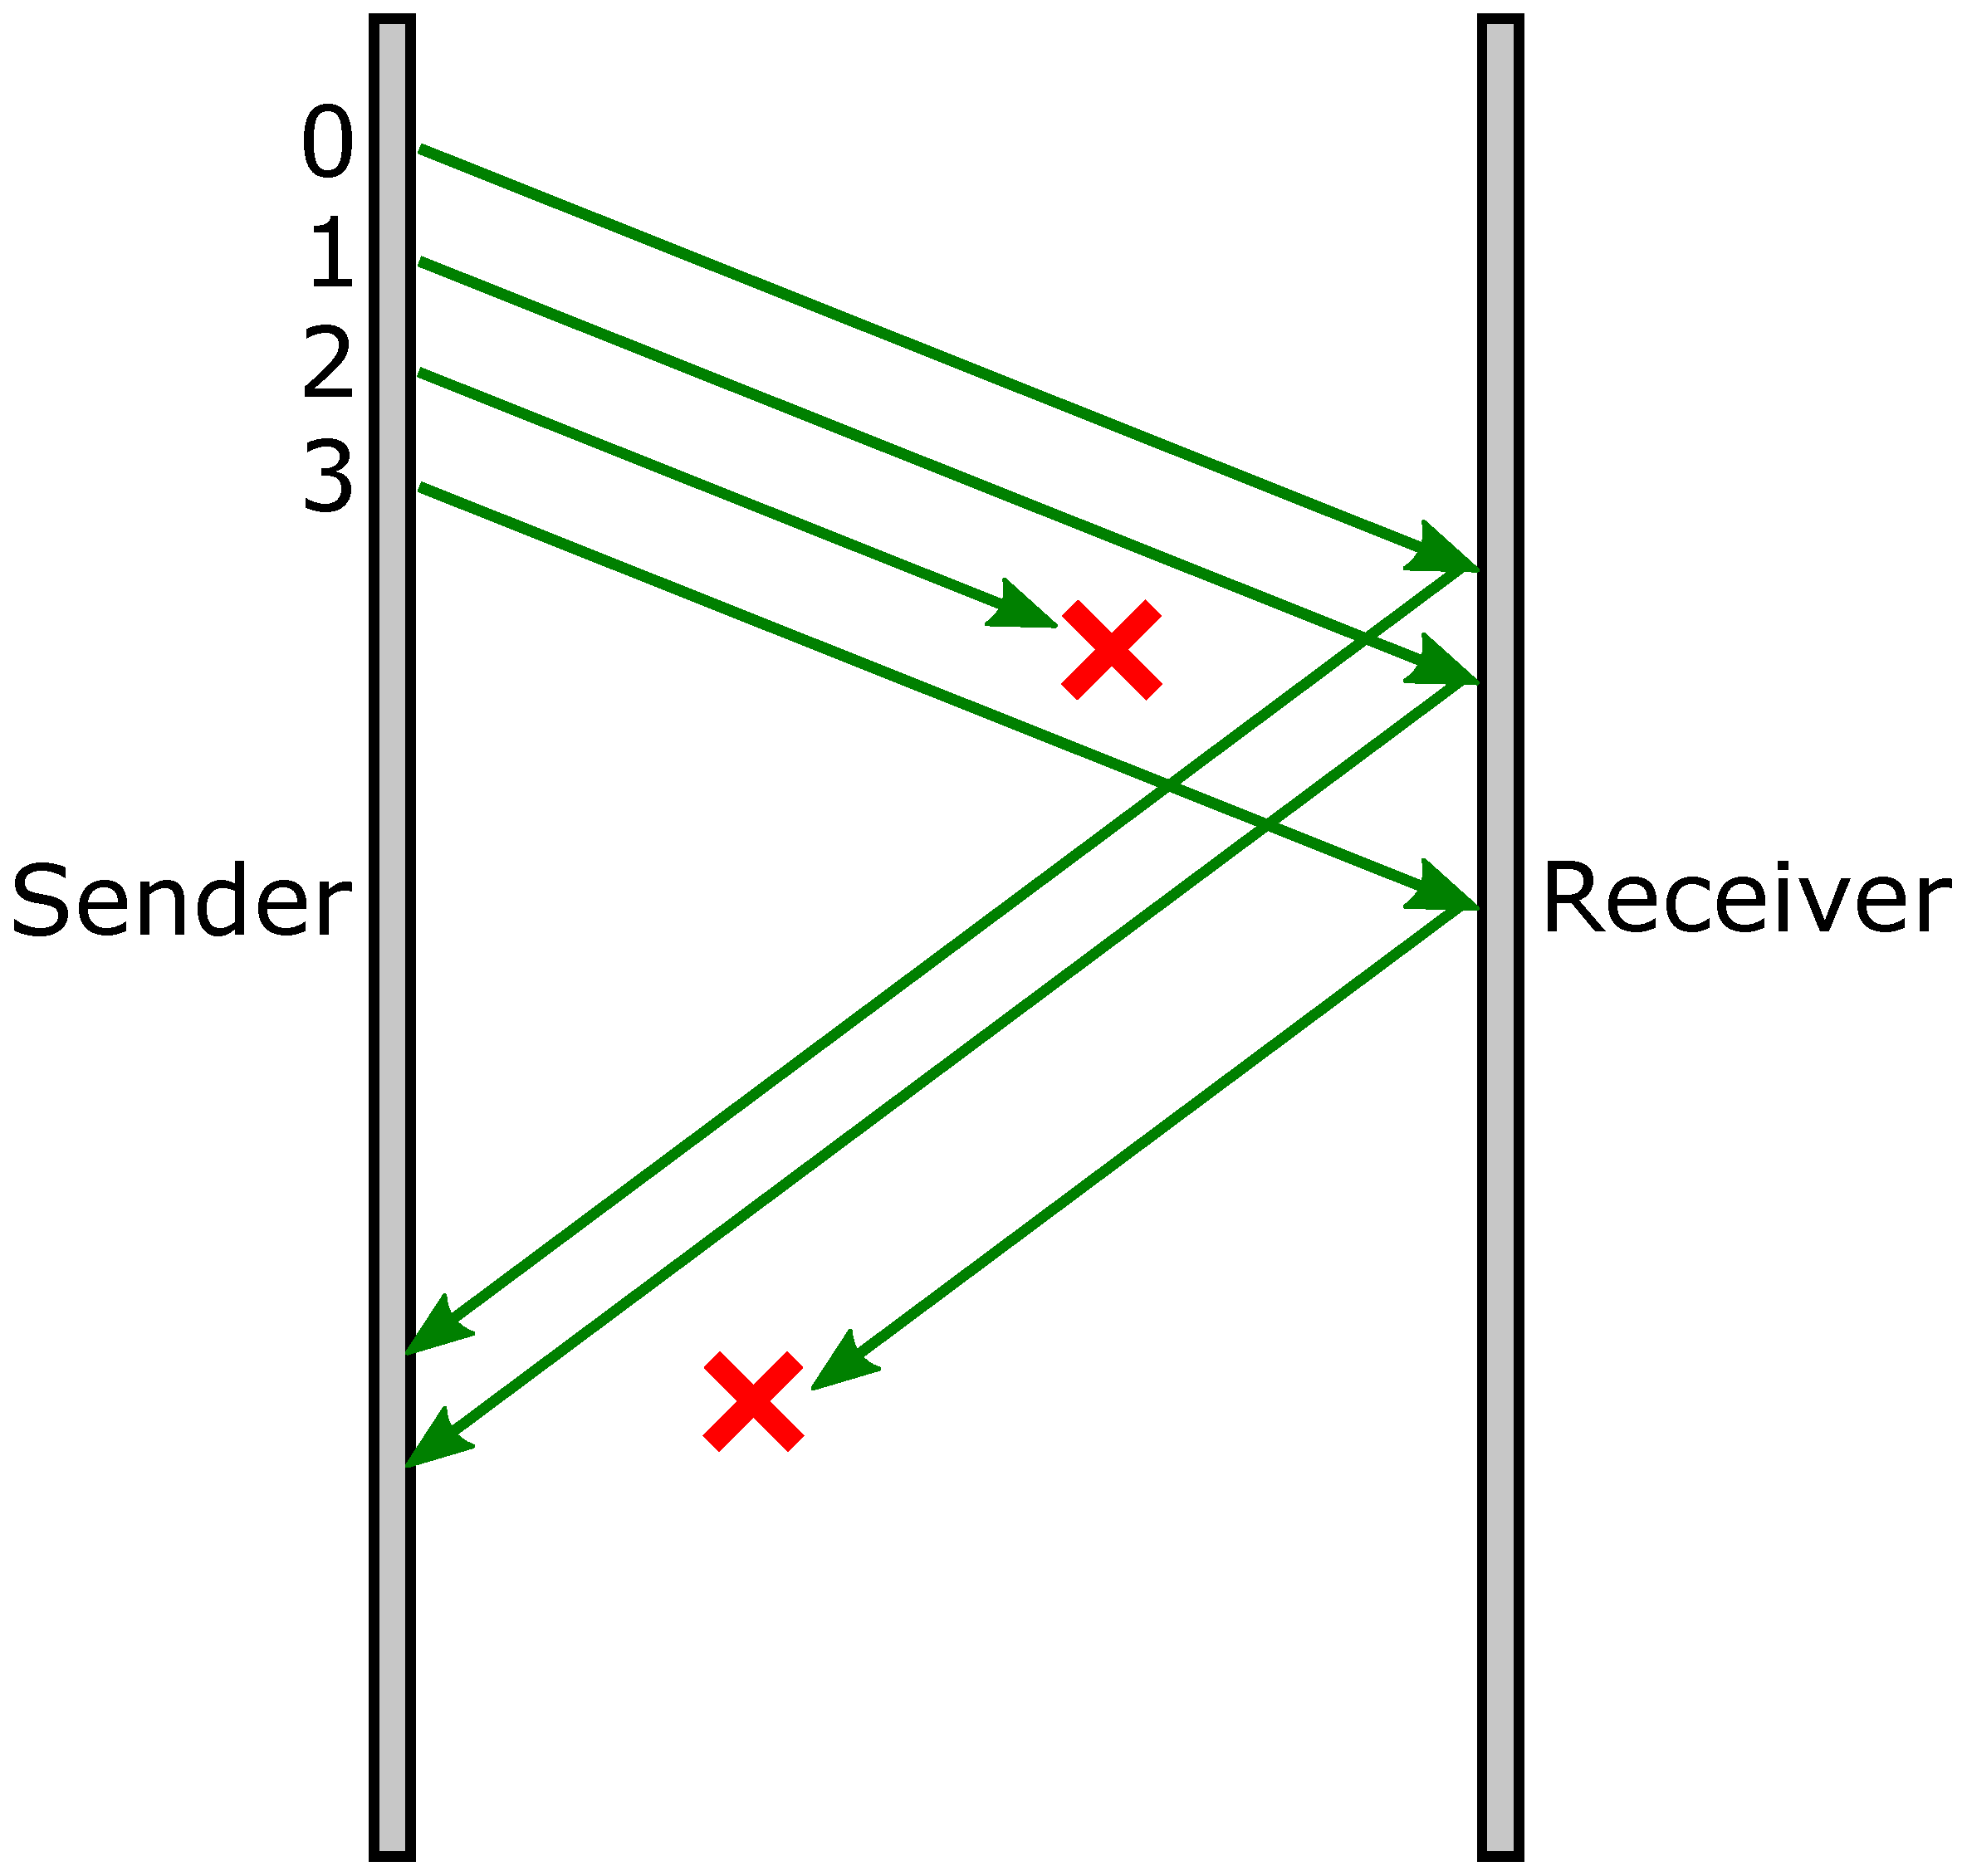
\includegraphics[width=80mm]{Q3.eps}
\end{figure}
\newpage
سوال 4) شکل زیر، مربوط به سازوکار \lr{Congestion Control} یک فرستنده‌ی TCP است. محور عمودی cwnd و محور افقی \lr{Transmission Round} را نشان می دهد.
\begin{figure}[htb]
\centering
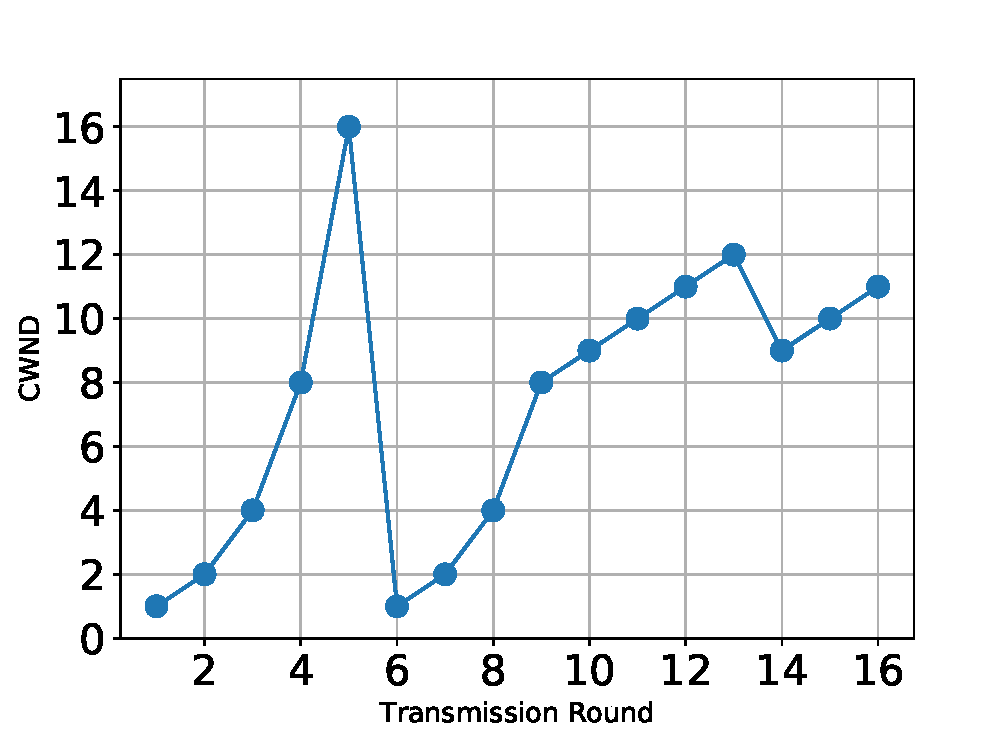
\includegraphics[width=100mm]{Q5.eps}
\end{figure}

الف) از کدام سازوکار (\lr{Tahoe} یا \lr{Reno}) استفاده شده است؟

ب) در کدام مراحل، فرستنده در حالت \lr{Slow Start} قرار دارد؟

پ) در کدام مراحل، فرستنده در حالت \lr{Congestion Avoidance} قرار دارد؟

ت) مقدار ssthresh در ارسال اول چند است؟

ث) در ارسال 14، فرستنده در چه حالتی است؟

ج) بین ارسال 5 و 6، گم شدن بسته به علت timeout بوده است یا \lr{3-duplicate-ACK}؟ چرا؟
\newpage
سوال 5) در \lr{Autonomous System} زیر، با فرض آن که نود A نود مبدا باشد:
\begin{figure}[htb]
\centering
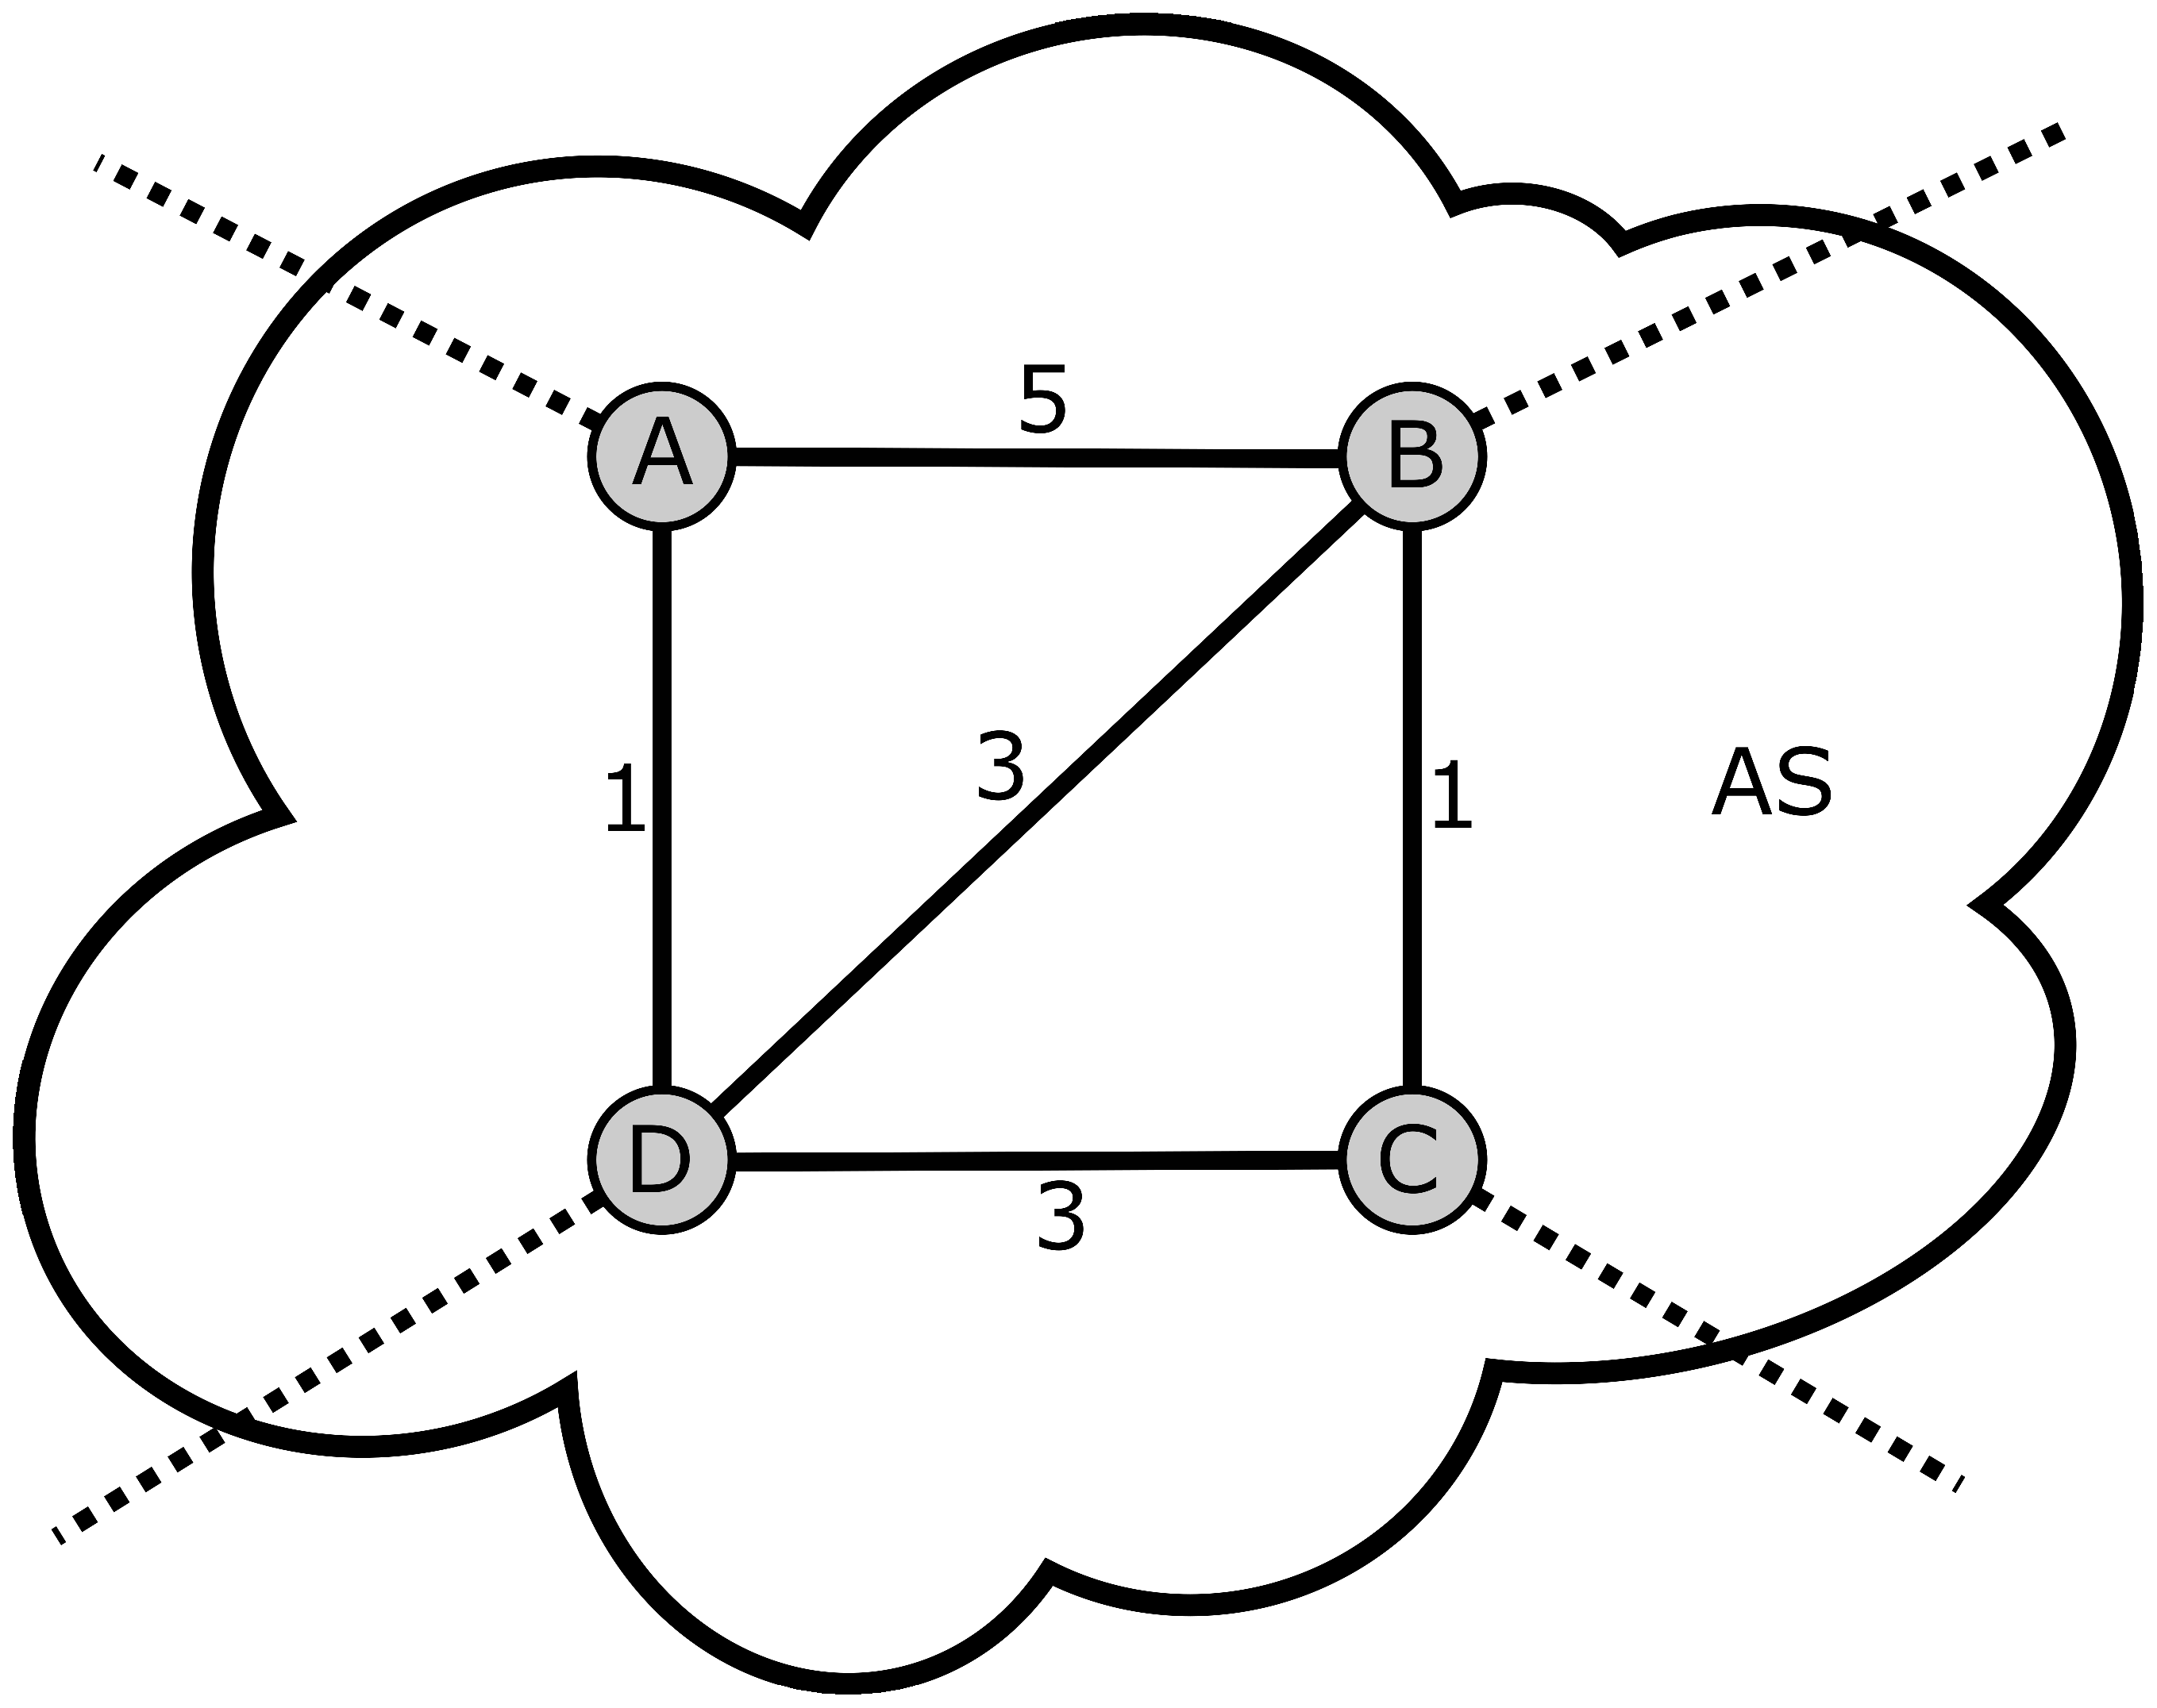
\includegraphics[width=100mm]{Q4.eps}
\end{figure}

الف) هر دو الگوریتم OSPF و RIP را برای یافتن کوتاهترین مسیر از نود A تا سایر نودها بیابید.

ب) فرض کنید نود A بخواهد بسته‌ی 1Kbytes را به سایر نودها Broadcast کند. میزان کل حجم بسته ای مبادله شده در تمام لینک های شبکه را چنانچه رویکرد 
\lr{Controlled Flooding with Reverse Path Forwarding}
اتخاذ شده باشد، محاسبه کنید.
%\newpage
%سوال 4) در شبکه ای با توپولوژی زیر، فرض کنید نود A می خواهد بسته ای به حجم 
%\lr{5 Kbytes}
%را به سایر نودها پخش 
%(\lr{Broadcast})
%کند. چه مقدار حجم داده در تمام لینک های شبکه استفاده خواهد شد اگر برای 
%\lr{Broadcast}
%کردن:
%
%الف) از
%\lr{Uncontrolled Flooding}
%استفاده شود؟
%
%ب) از
%\lr{Controlled Flooding}
%با روش 
%\lr{reverse path forwarding}
%استفاده شود؟
%
%پ) از 
%\lr{Minimum Spanning Tree}
% با روش 
%\lr{center-based}
%استفاده شود؟ (همچنین مراحل ساخت درخت را توضیح دهید.)
%
%(هزینه تمام لینک ها برابر 1 است)
%\begin{figure}[htb]
%\centering
%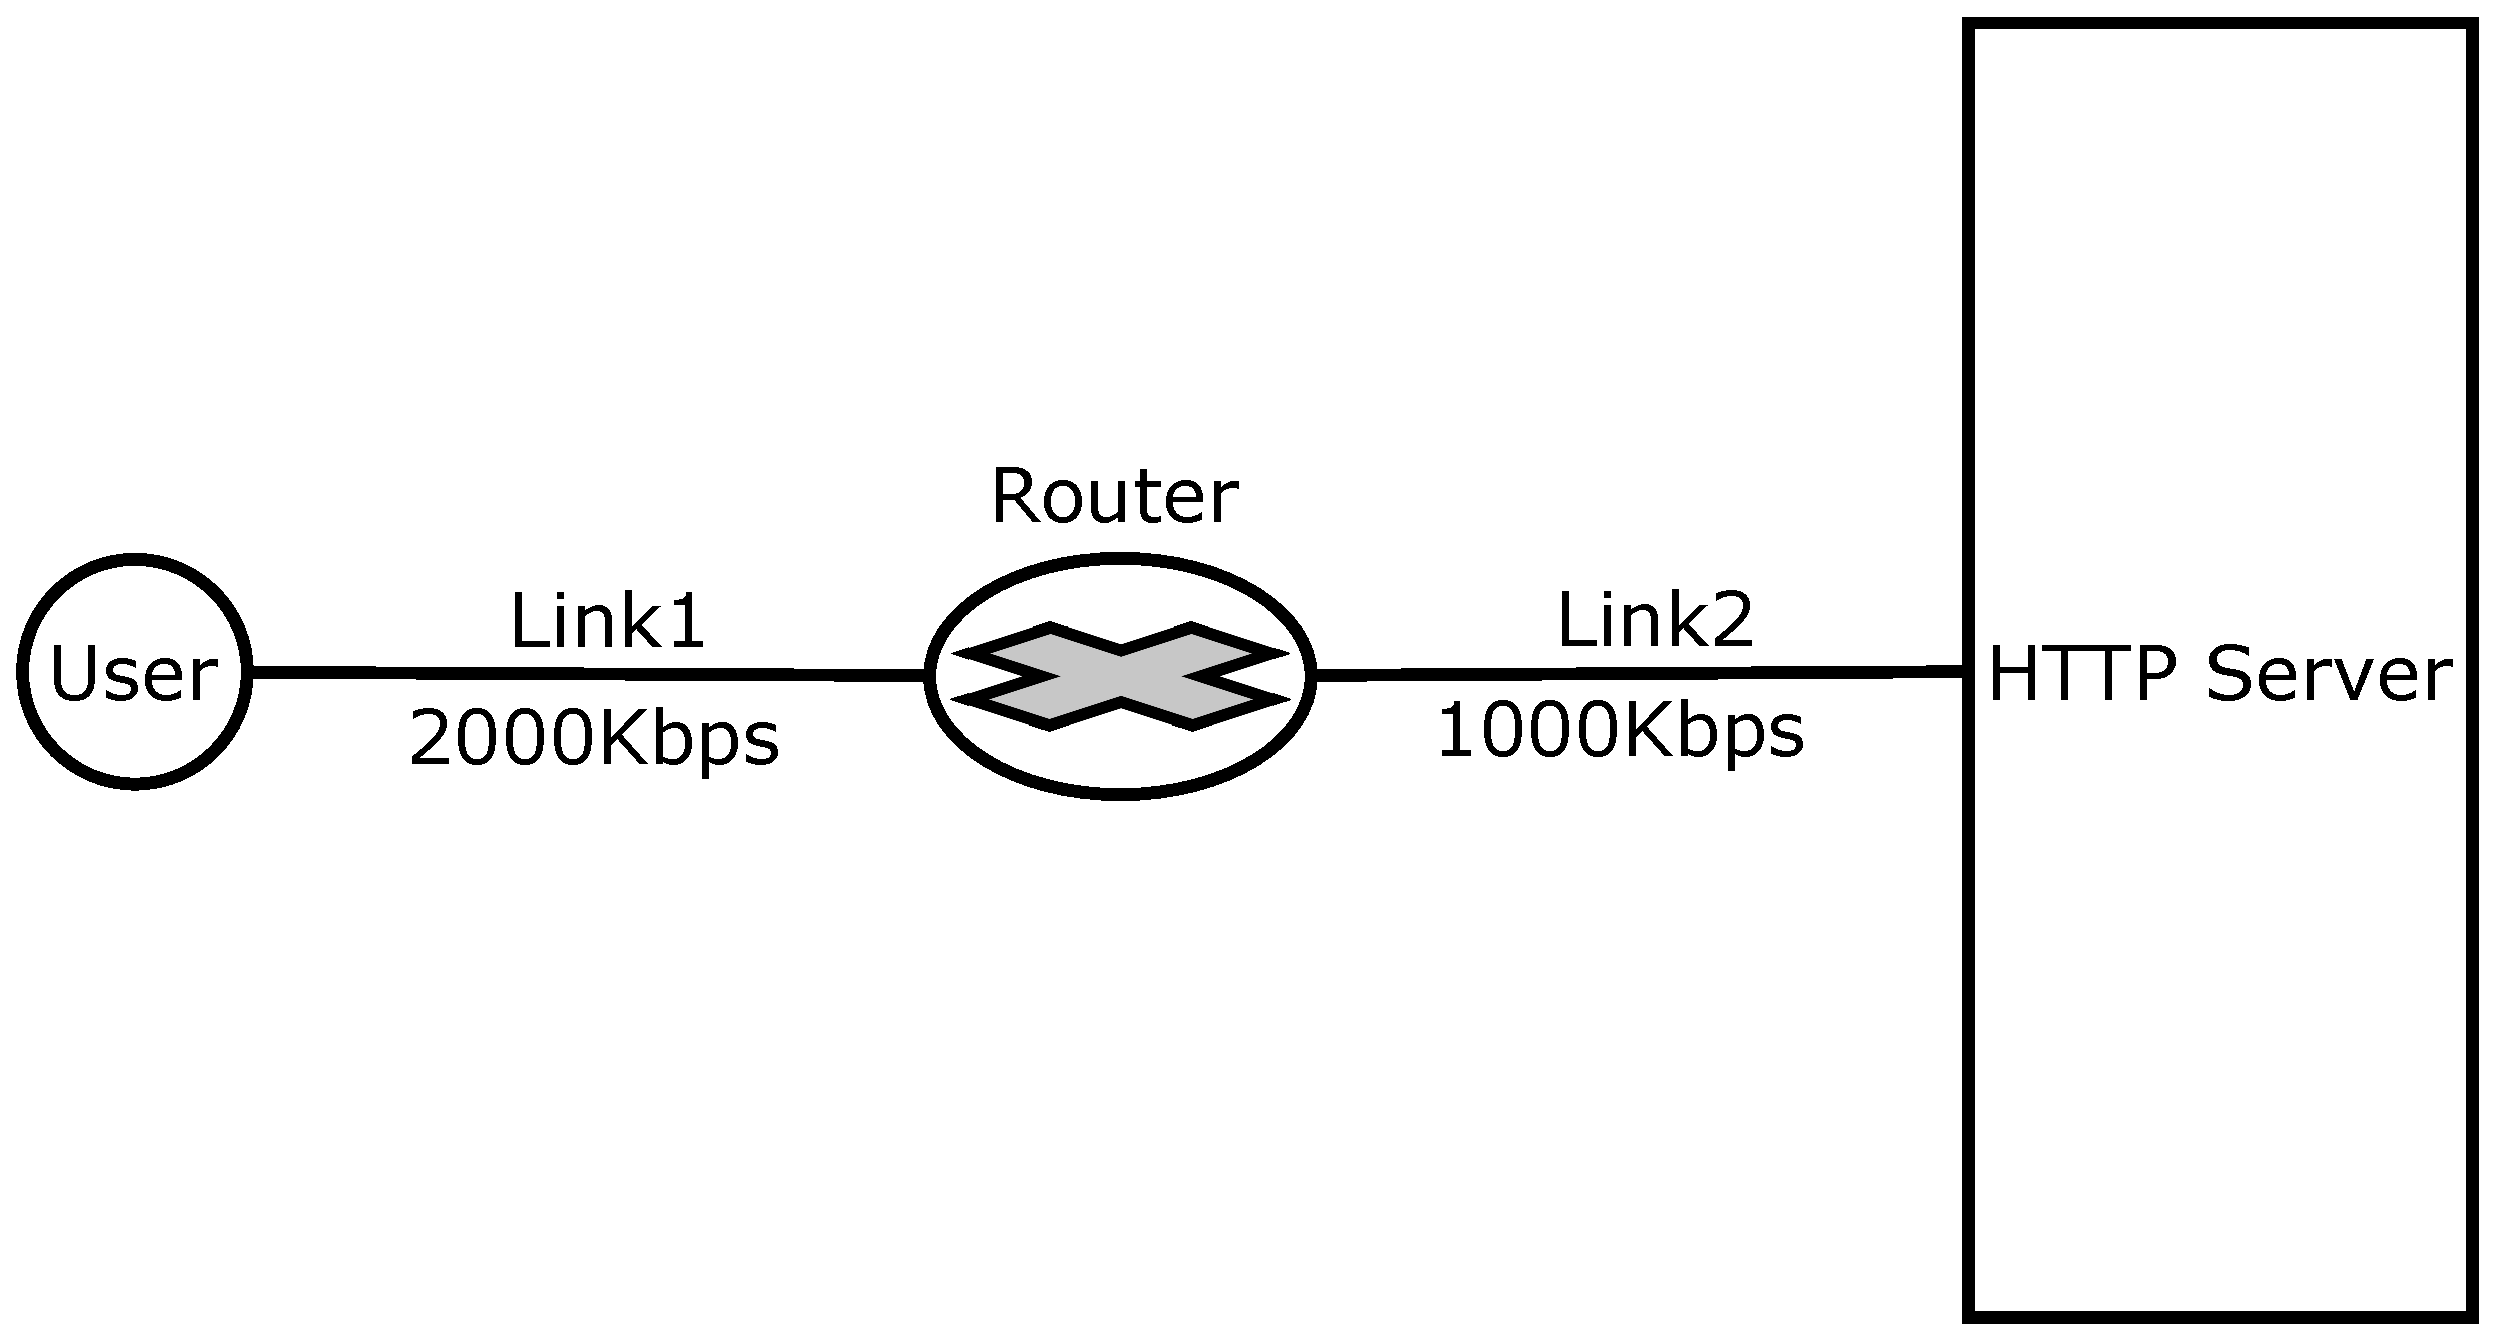
\includegraphics[width=130mm]{Q2}
%\end{figure}
%\newpage
%سوال 5) در دیاگرام فضا-زمان زیر برای پروتکل
%\lr{CSMA/CD}
%، دو نود B و D پس از آشکار سازی تصادم بسته‌ها 
%(\lr{Collision Detection})
%، از روش 
%\lr{binary exponential backoff}
%برای تعیین زمان تصادفی ارسال خود استفاده می کنند. نودها پس از اندازه گیری 
%$
%n
%$
%تصادم بسته‌ی خود، زمان تصادفی ای در بازه‌ی 
%$
%\{0,1,2,\cdots,2^{n}-1\}\times 1msec
%$
%مستقل از هم انتخاب کرده و پس از سپری شدن زمان انتخاب شده‌ی خود، اقدام به ارسال مجدد بسته ها می کنند. اگر هر نود برای ارسال هر بسته‌ی خود به 1 میلی ثانیه زمان نیاز داشته باشد،
%
%الف) 
%%با چه احتمالی نود $B$، 2 بار 
%%\lr{collision}
%%را برای بسته‌ی خود تجربه می کند و در بار سوم موفق به ارسال بسته می شود؟
%با چه احتمالی نود $B$ پس از 1 بار تجربه کردن
%\lr{collision}
%،  در بار دوم موفق به ارسال بسته می‌شود؟
%
%ب) احتمال اینکه هر دو نود در 5 ارسال اول دچار 
%\lr{collision}
%شوند، چقدر است؟
%
%(فرض کنید هر دو نود در زمان صفر اقدام به ارسال بسته‌ی خود می کنند و تصادم اول رخ می‌دهد. هر نود پس از ارسال موفق هر بسته، بلافاصله ارسال بسته‌ی بعدی را شروع می کند. همچنین سایر تاخیرها از جمله تاخیر 
%\lr{collision detection}
%را صفر در نظر بگیرید.)
%\begin{figure}[htb]
%\centering
%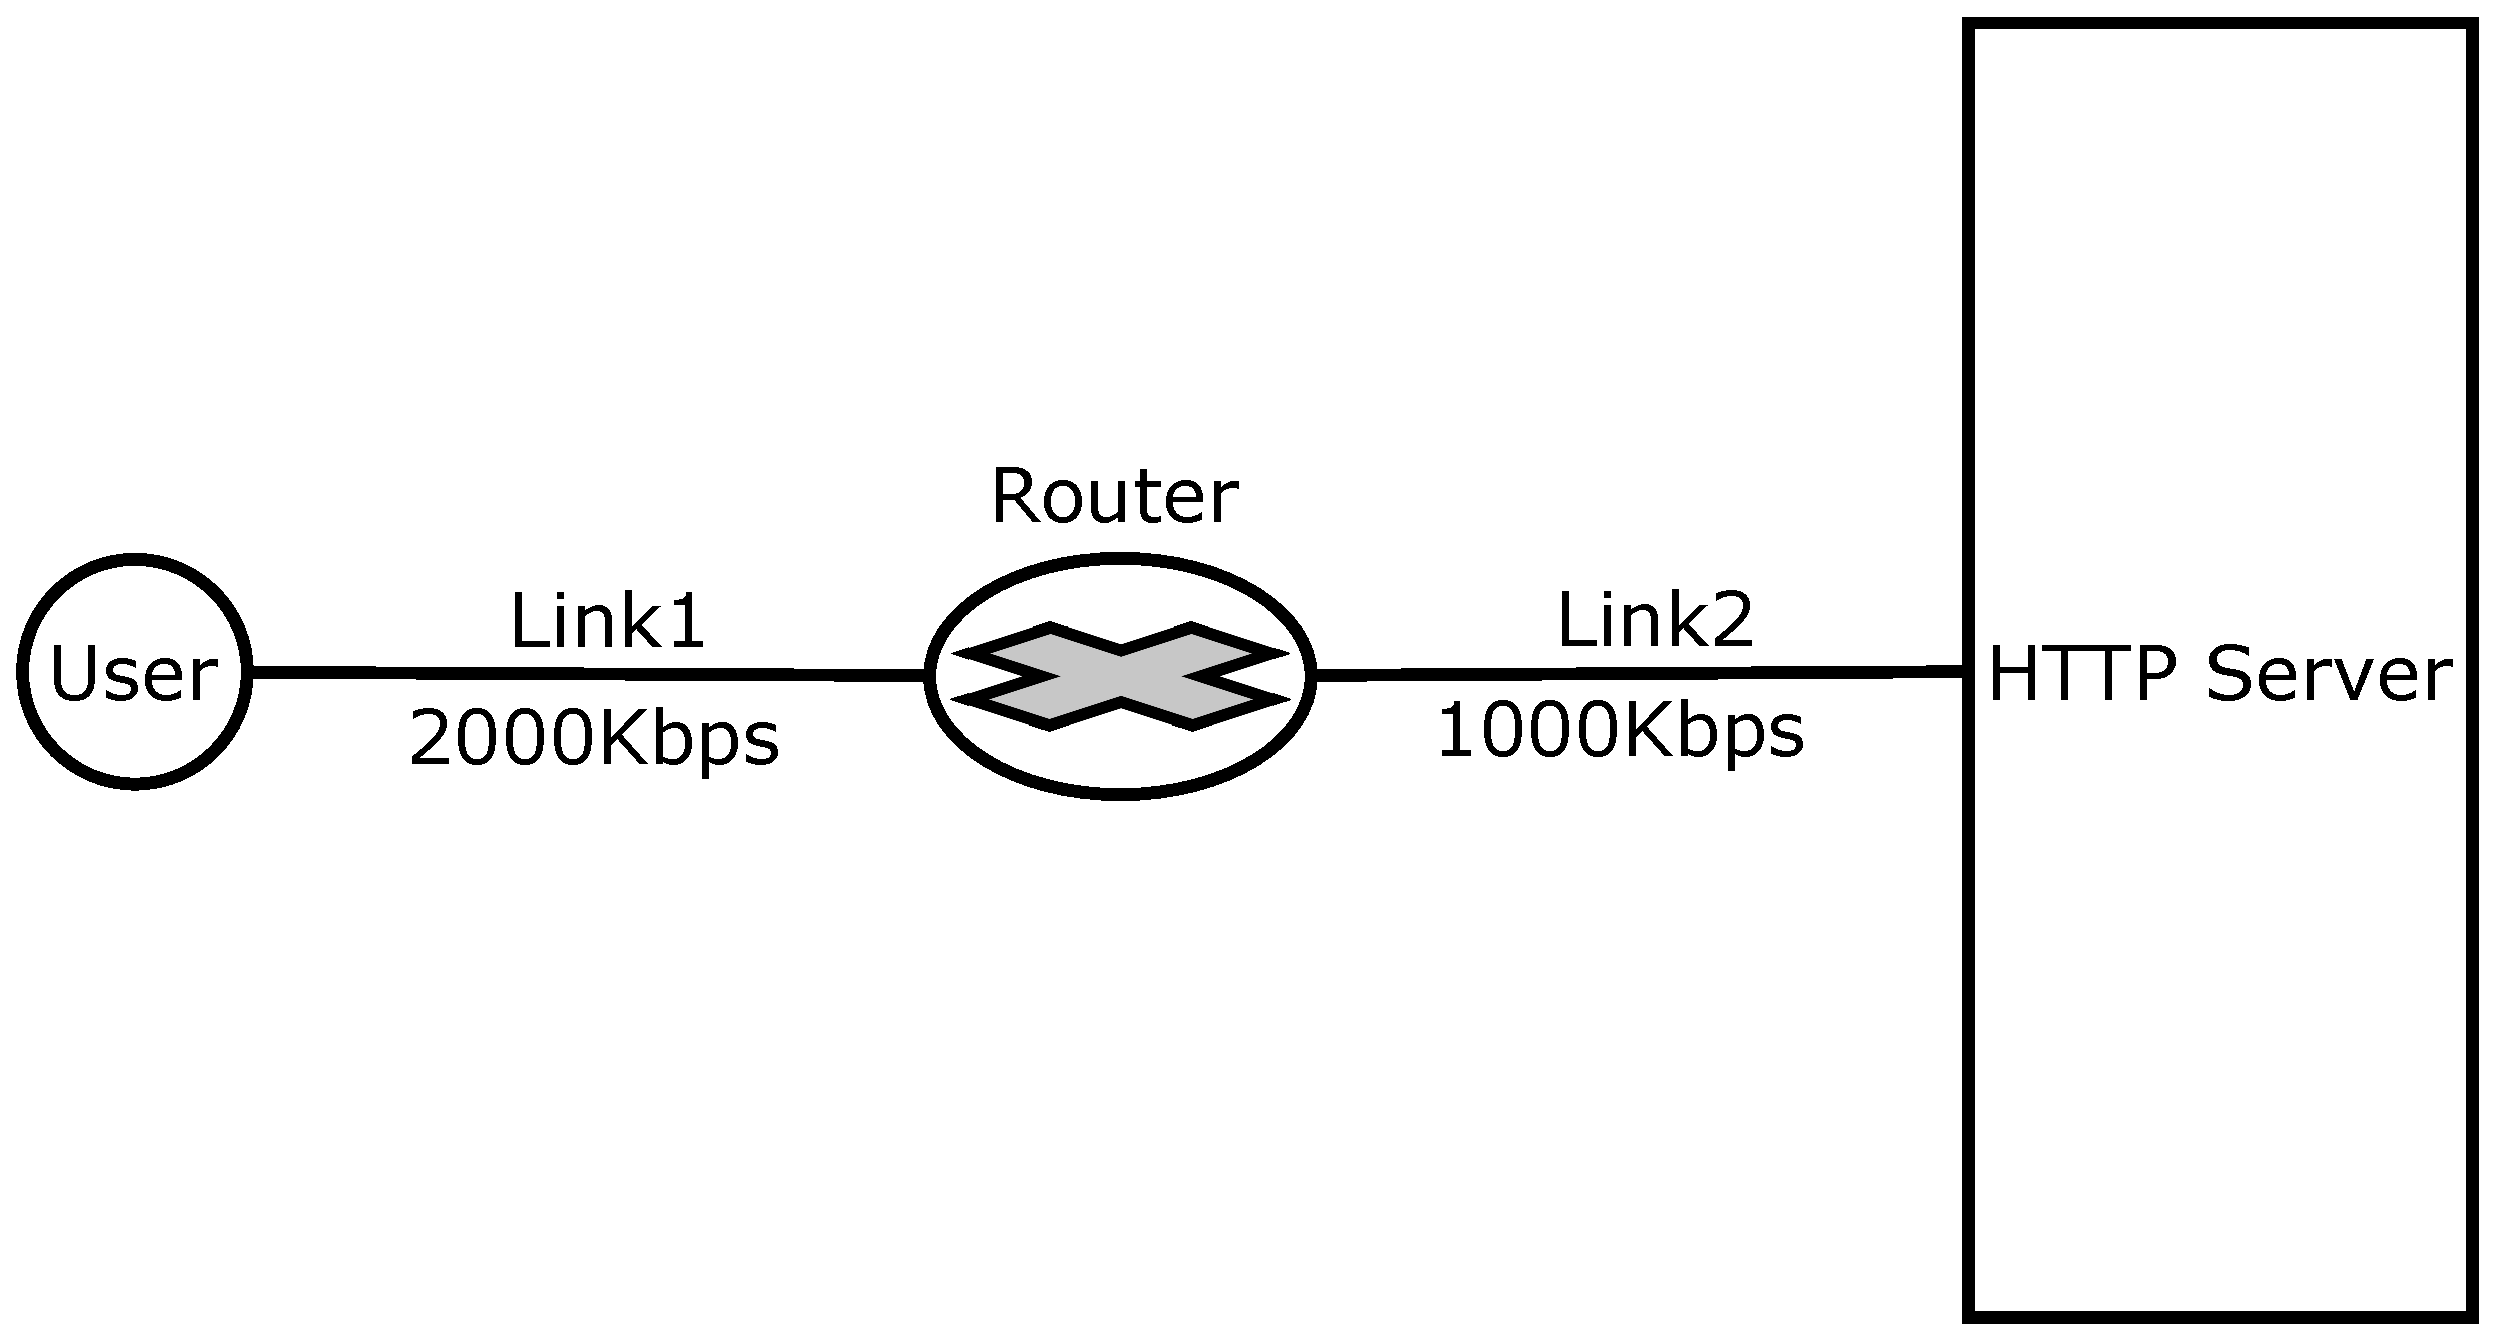
\includegraphics[width=130mm]{Q2}
%\end{figure}
\end{document}